\documentclass[12pt]{article} 

\usepackage[utf8]{inputenc} 
\usepackage{geometry} 
\geometry{letterpaper} 
\usepackage{hyperref}
\usepackage{verbatim}
\usepackage{enumitem}
\usepackage{fancyhdr} 
\usepackage{tikz}
\usepackage{tikz-qtree}
\usepackage{ulem}
\usepackage{fourier}

\pagestyle{fancy} 
\renewcommand{\headrulewidth}{0pt} 
\lhead{}\chead{}\rhead{}
\lfoot{}\cfoot{\thepage}\rfoot{}

\title{\vspace{-60pt}Ling 201 syntax practice problems}
\author{\vspace{-40pt}}
\date{\vspace{-60pt}}
\begin{document}
\maketitle

\section{Rules}

S $\rightarrow$ NP VP\\
NP$\rightarrow$ (D) (A) N (PP) \\
VP$\rightarrow$ V (NP) (PP) \\
PP$\rightarrow$ P (NP)

\section{The British left waffles on Gibraltar.}

\subsection*{First parse:}

\vspace{200pt}

\subsection*{Second parse:}

\pagebreak

\section{Enraged cow injures farmer with ax.}

\subsection*{First parse:}

\vspace{250pt}

\subsection*{Second parse:}

\pagebreak

\section{I saw a man on a hill with a telescope.}


\subsection*{First parse:}

\vspace{175pt}

\subsection*{Second parse:}

\vspace{175pt}

\subsection*{Third parse:}

\pagebreak

\section{Answers}

\subsection*{The British left waffles on Gibraltar.}

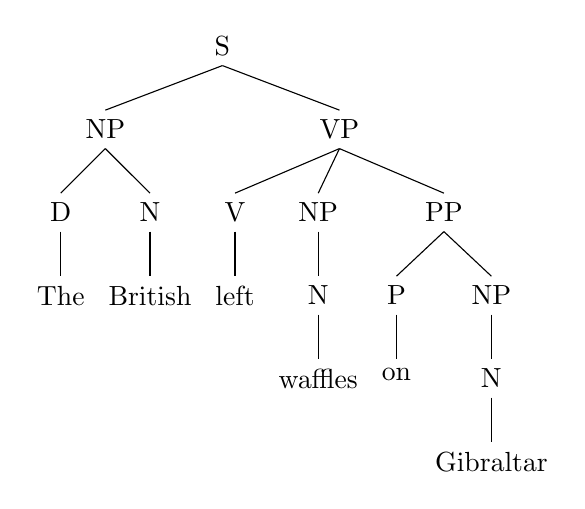
\begin{tikzpicture}
\tikzset{every tree node/.style={align=center,anchor=north}}
\Tree  [.S [.NP [.D The ] [.N British ] ] [.VP [.V left ] [.NP [.N waffles ] ] [.PP [.P on ] [.NP [.N Gibraltar ] ] ] ] ]
\end{tikzpicture}

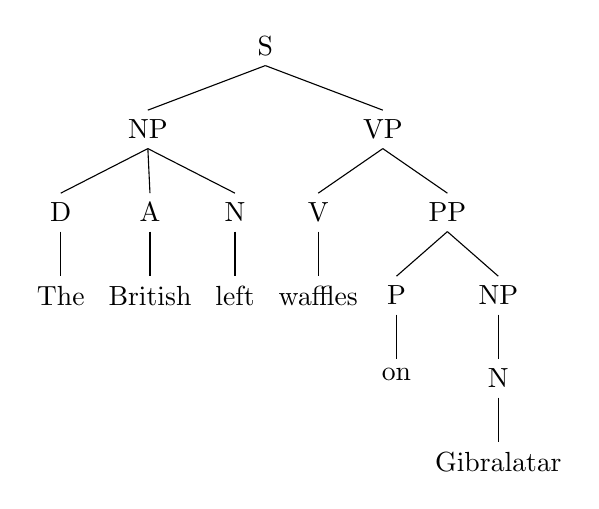
\begin{tikzpicture}
\tikzset{every tree node/.style={align=center,anchor=north}}
\Tree  [.S [.NP [.D The ] [.A British ] [.N left ] ] [.VP [.V waffles ] [.PP [.P on ] [.NP [.N Gibralatar ] ] ] ] ] 
\end{tikzpicture}

\subsection*{Enraged cow injures farmer with ax.}

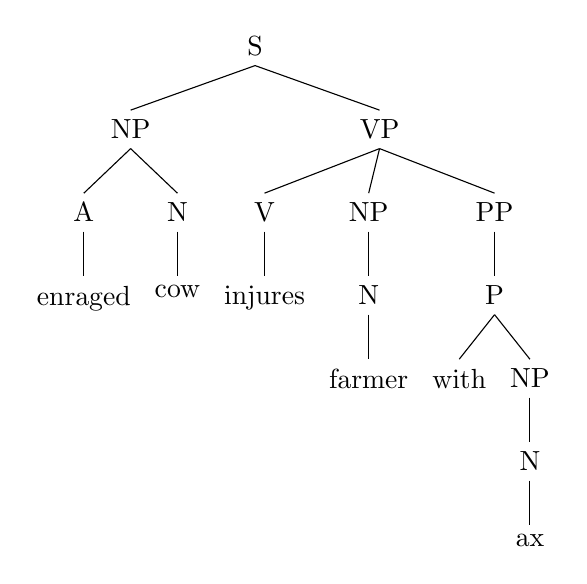
\begin{tikzpicture}
\tikzset{every tree node/.style={align=center,anchor=north}}
\Tree  [.S [.NP [.A enraged ] [.N cow ] ] [.VP [.V injures ] [.NP [.N farmer ] ] [.PP [.P with [.NP [.N ax ] ] ] ] ] ]
\end{tikzpicture}

\begin{tikzpicture}
\tikzset{every tree node/.style={align=center,anchor=north}}
\Tree  [.S [.NP [.A enraged ] [.N cow ] ] [.VP [.V injures ] [.NP [.N farmer ] [.PP [.P with [.NP [.N ax ] ] ] ] ] ] ]
\end{tikzpicture}

\subsection*{I saw a man on a hill with a telescope.}

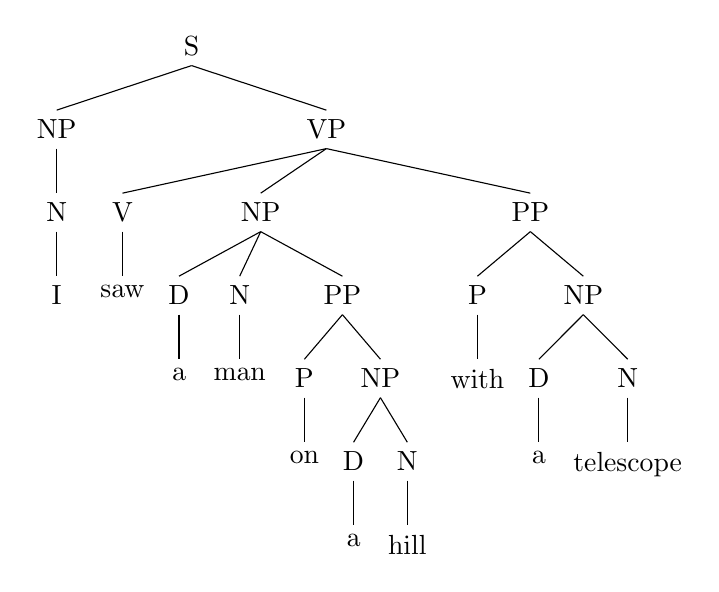
\begin{tikzpicture}
\tikzset{every tree node/.style={align=center,anchor=north}}
\Tree  [.S [.NP [.N I ] ] [.VP [.V saw ] [.NP [.D a ] [.N man ] [.PP [.P on ] [.NP [.D a ] [.N hill ] ] ] ] [.PP [.P with ] [.NP [.D a ] [.N telescope ] ] ] ] ] ] ]
\end{tikzpicture}

\begin{tikzpicture}
\tikzset{every tree node/.style={align=center,anchor=north}}
\Tree  [.S [.NP [.N I ] ] [.VP [.V saw ] [.NP [.D a ] [.N man ] [.PP [.P on ] [.NP [.D a ] [.N hill ] [.PP [.P with ] [.NP [.D a ] [.N telescope ] ] ] ] ] ] ] ]
\end{tikzpicture}

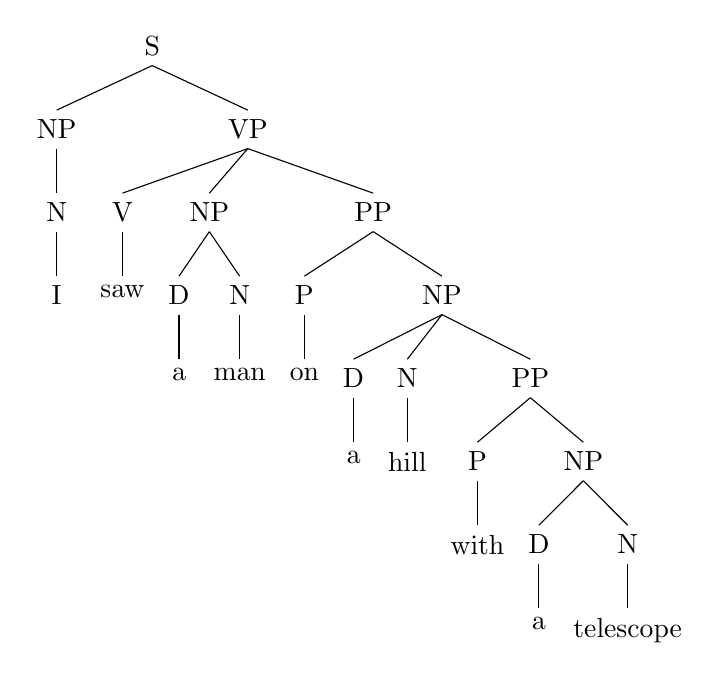
\begin{tikzpicture}
\tikzset{every tree node/.style={align=center,anchor=north}}
\Tree  [.S [.NP [.N I ] ] [.VP [.V saw ] [.NP [.D a ] [.N man ] ] [.PP [.P on ] [.NP [.D a ] [.N hill ] [.PP [.P with ] [.NP [.D a ] [.N telescope ] ] ] ] ] ] ]
\end{tikzpicture}

\end{document}
